\documentclass[reqno]{amsbook}
\usepackage[utf8]{inputenc}
\usepackage{HBSuerDemir}
\usepackage{caption}
\usepackage{wrapfig}

\begin{document}

    \hPage{b1p2/21}
    \footnote{I have used [reqno] in "documentclass" options in order to align the equation numbers right, instead of left(as default)}
    \indent 1. \underline{Integral test} (of McLAURIN):
    \begin{thm}{Fibration}
        Let $\sum_{p}^{\infty} a_{n}$ be a series of positive term with
        $a_{n} = f(n)$ and $D_{f} = [p, \infty)$. If $f(x)$ is positive, continuous and decreasing on $[N, \infty)$, N$>$p, then
        \[
            \sum_{p}^{\infty} a_{n} \quad \textrm{and}\quad \int_{N}^{\infty} \! f(x) \, \hDif x\\
        \]
        are both convergent or both divergent.
    \end{thm} \footnote{The theorem in my page was unnumbered but Mr. Bingöl told me to use theorems as default}
    \begin{proof}
        Consider the partial sum $s_{n}$. Separating from it the terms $a_{p},  \dotsc, a_{N-1}$ of $[p, N-1]$ on which $f(x)$ may not satisfy the hypothesis, we set
        \begin{equation}
            s_{n} = s_{N-1} + \underbrace{a_{N} + \cdots + a_{n}}_{s_{n}^\prime} \tag{s_{N-1} \quad is\quad finite}
        \end{equation}
        $\lim s_{n}$ exists if $\lim s_{n}^\prime$ exists. Then the series is convergent, otherwise divergent.
    \end{proof}
    \begin{wrapfigure}{r}{0.4\linewidth}
        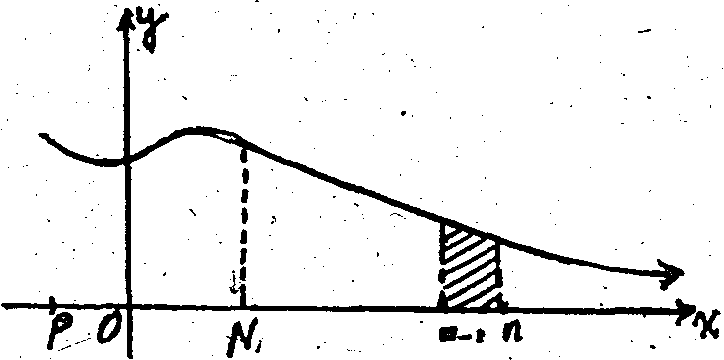
\includegraphics[width=\linewidth]{images/b2p1-021-fig01.png}
        \caption*{}
        \label{b1p2/21: Figure 1}
    \end{wrapfigure}
    \footnote{I used "wrapfig" package in order to align the figure and text properly}
    \footnote{I used "caption" package in order to delete the caption of figure}
    \indent Consider the graph of $f(x)$. \\$f(x)$
    being decreasing, one has the double inequality\\
    \begin{center}
        $f(n)<\int_{n-1}^{n} \! f(x) \, \hDif x < f(n-1)$\\~\\
    \end{center}
    which, when written for all subintervals on $[N, n]$ and added gives\\
    \[
        {s_{n}^\prime} - s_{N} < \int_{N}^{n} \! f(x) \, \hDif x < s_{n-1}^\prime - s_{N-1}
    \]
    \indent If the integral has a limit when $n \to \infty$, this limit is an upper bound for the increasing sequence $({s_{n}^\prime} - s_{N})$. Then $({s_{n}^\prime})$ and hence $\sum_{p} a_{n}$ is convergent.\\
    \indent If the integral diverges to $\infty$ the same is true for $(s_{n-1}^\prime - s_{N-1})$. Then $(s_{n-1}^\prime)$ and hence $\sum_{p}^{} a_{n}$ is divergent.

\end{document}